\subsection{Existing Solutions} \label{sec:existingSolutions}

Traditionally, edge devices were isolated cluster heads mainly forwarding traffic from their slaves to the cloud. Today, they are an integral part of the data flow pre-processing data and executing part of the business logic. But, there are still no coherent architectural as well as technological standards. In this section we will compare widely adopted and developed solutions in the industry to detect similarities and differences. The solutions also differ in age and 

% https://scholar.google.com/scholar?cluster=13680069378267225814&hl=de&as_sdt=0,5
% https://www.pac-online.com/sites/pac-online.com/files/upload_path/PDFs/Thema_des_Monats_Juni_2017_IoT_Plattformen.pdf
% https://blog.bosch-si.com/bosch-iot-suite/lessons-learned-using-kubernetes-in-iot-deployments/

\subsubsection{Bosch IoT Gateway Solutions}
\comment{https://www.bosch-iot-suite.com/service/gateway-software/}
The Bosch IoT Gateway Software\cite{BoschIoT13:online} is the "oldest" software analyzed. It is based on the OSGi technology\cite{osgiDefintion25:online}, which is an aliance driven project from the Open Services Gateway initiative (OSGi). It defines a set of specifications (with reference implemetation and tests) for a dynamic modular system based on so called bundles, third party software, running on the Java Virtual Machine (JVM)\footnote{This means it is possible to use other languages apart from Java which can run in a JVM, e.g. Kotlin.}. It is important to note that Bosch also supplies a cloud part which is based on Kubernetes.\\
The OSGi framework consists of a layered model shown in \cref{fig:osgiLayerModel}. 
\begin{figure}[h!]
    \centering
    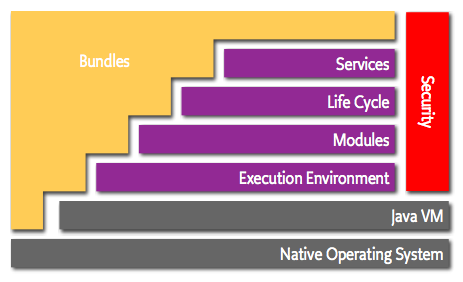
\includegraphics[scale=0.8]{figures/layering-osgi.png}
    \caption{From the official OSGI documentation\cite{osgiFrameworkArchitec22:online}.}
    \label{fig:osgiLayerModel}
\end{figure}
The Service layer interconnects the bundles making it possible for them to communicate via plain old java objects (POJO).The Life-Cycle layer handles the the state of the application (start, stop, update and uninstall). The Modules layer defines how an application can import and export code and the Execution Environemnt defines which methods and classes are available in a specific environemnt. Finally, the Security layer encompasses all other layers and handles for example code authentication, the digital signing of jar files, file access restrictions, certificates and more.\\
To the authors best knowledge there are currently five frameworks implementing the OSGi model besides the Bosch IoT Gateway Software\cite{BoschIoT13:online}. In a blog entry from 2015 Bosch compares the OSGi technology to other gateway solutions and says it "is the only one with clearly defined specs and an open specification process behind them"\cite{boschBlogOSGi69:online}. Boschs solution is proprietary and tailor made for edge-computing devices with IIoT in mind\cite{OSGiforIoTBlog27:online}. It runs on Linux, Windows, mac OS, Android, and VxWorks and according to Bosch more than 40 different gateway devices\cite{BoschIoT13:online}. The software is stable at major version 9 and still under heavy development. It is presented as exemplary software by the OSGi Alliance for IoT Gateways \cite{exampleIoTGateweOSGi:online} and thus used in this report. \Cref{fig:boschIoTGatewaySetup} shows where Boschs IoT solution is situated in the IoT environment. Bosch provides the OSGi framework implementation for the gateways and additional features for the cloud to ease the management of the gateways and store the accumulated data.
\begin{figure}[h!]
    \centering
    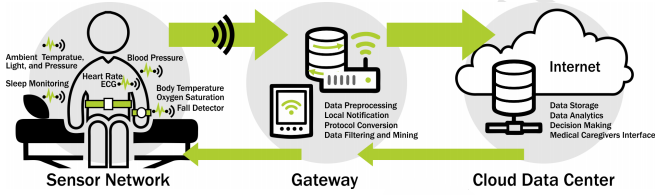
\includegraphics[scale=0.8]{figures/iotSetup.png}
    \caption{From the official Bosch documentation \cite{BoschIoT13:online}.}
    \label{fig:boschIoTGatewaySetup}
\end{figure}
Moreover, it supports a wide variety of communication protocls, BLE, ZigBee and MQTT, just to name a few. The main restriction is the JVM support for a protocol.  

\subsubsection{ioFog}
ioFog is one of the older projects in this report, with the first official release in 2016\cite{ioFogMainBlog:online}. Similarly to the OSGi framework it provides a runtime environment for applications, mainly intended for microservices. In addition, it includes a message bus, dynamic configuration of the microservices, and remote debugging\cite{ioFogMainBlog:online}. It runs on (almost) all Linux distributions and only requires Docker to be installed. In their official system requirements they only recommed using a Raspberry Pi as a worker node and not to run the Controller and Connector infrastructure \cite{ioFOgQuickStart:online}.
\Cref{fig:ioFogComponent} shows the fog computing layers in more detail.
\begin{figure}[h!]
    \centering
    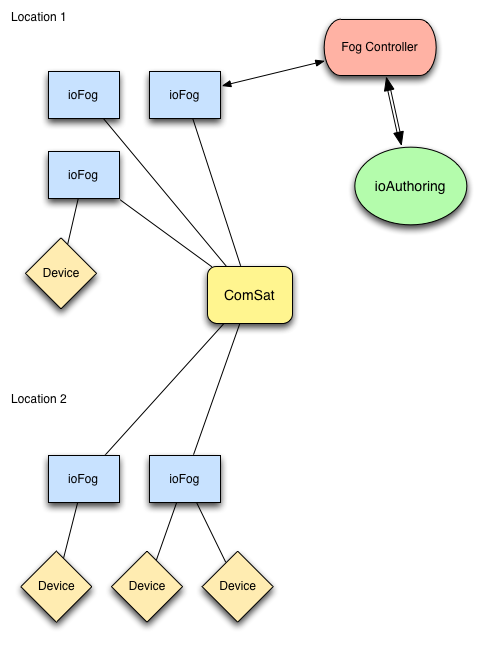
\includegraphics[scale=0.4]{figures/ioFog-Component_Diagram.png}
    \caption{hallo}
    \label{fig:ioFogComponent}
\end{figure}\\
The ioAuthoring application and the ioFog instances provide orchestration and management of the microservices. They are the main interaction points between the administrator and the system.
The fog computing software agent, called "ioFog", runs on various operating systems and provides a universal runtime for the IoT microservices. It includes a Software Development Kits (SDKs) in multiple programming languages to provide developers with the convenience of programming against standardized objects. The communication between different ioFog instances is facilitated through an internetworking utility that runs on popular Linux distributions, called "ComSat". Finally, for testing a tool for mimicking the fog computing runtime is included as well.\\
In a recent blog post from Mike Milinkovich, the Executive Director of the Eclipse Foundation Inc., he announced the initial availability of ioFog features that make any Kubernetes distribution edge-aware. He continuous saying that "these native Kubernetes enhancements are in the process of being contributed to the Eclipse ioFog open source project.", so not all features are available in the stable release as of the time of writing. But essentially, the ioFog Kubernetes APIs would provide standardized way of communication between the Kubernetes API Server and the ioFog instance.

\subsubsection{Docker Edge Solution}
Docker is commonly known for its containerization software and is often confused with the containers themselves (like google for search). The core container runtime, containerd, was donated by Docker to the Cloud Native Computing Foundry (CNCF) in 2017\cite{containerDonationDocker79:online} which manages and develops it now. Now, the company Docker focuses on providing an ecosystem around containers making them easy to deploy, secure and replicate. Recently, Docker announced a new partnerships with ARM and  a new strategy for edge devices.\\
\Cref{fig:dockerEdge} shows the Docker Edge Solution in context. 
\begin{figure}[h!]
    \centering
    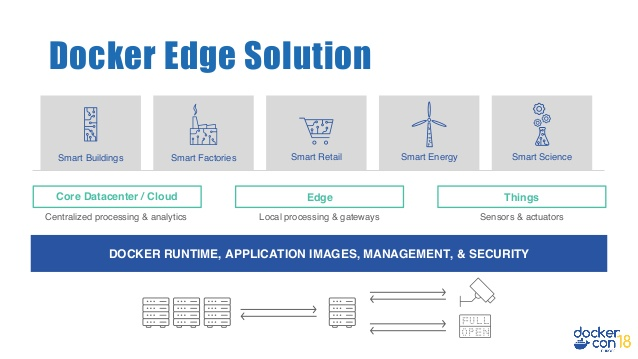
\includegraphics[scale=0.65]{figures/docker-edge-solution.jpg}
    \caption{Docker Edge solution .}
    \label{fig:dockerEdge}
\end{figure}
The solution consists of a few different products from its enterprise solution focusing on security, scalability/deployability and easy of use. The components are the same, but the edge focus is on fault tolerance and platform support, hence the new partnership with ARM. A core component of the suit is the docker registry, which can be mirrored/replicated on many difference servers for scaleability and fault tolerance. The edge registry can function without constant communication with the rest of the swarm. In case of no connection, the registry will only pull images which it already posses. As edge devices often have limitted disk space, docker only synchronizes promoted images on these nodes. Similarly to tags in git, promoted images are signed images that are explicitly marked as production ready. \cref{fig:dockerRegistryForIoT} shows registry management in the cloud (on the left) vs. on the edge (on the right).
\begin{figure}[h!]
    \centering
    \noindent\makebox[\textwidth]{
    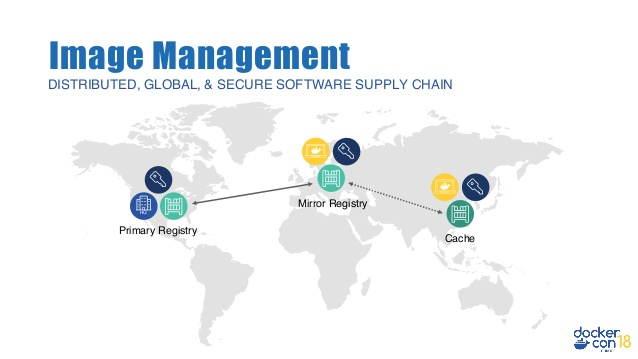
\includegraphics[width=(\textwidth+4cm)/2]{figures/docker-edge-computing-with-docker-enterprise.jpg}
    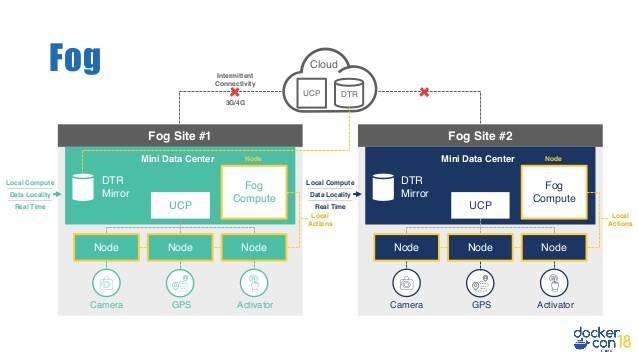
\includegraphics[width=(\textwidth+4cm)/2]{figures/docker-edge-registry-mirror.jpg}}
    \caption{The Docker registry in the cloud (left) vs. on the edge (right).}
    \label{fig:dockerRegistryForIoT}
\end{figure}
Whereas the cloud registry is build high availability (HA/LB) of the nodes in the swarm with fault tolerance against other nodes being unavailable, the edge registry is designed to have fault tolerance on it's own Internet access. In case of no connection it works as a standalone component, but synchronizes itself when it has a connection.\\
Importantly, the Docker Edge Solution is not a standalone solution, but integrates into the Docker ecosystem enabling remote management.

\subsubsection{K3s}
K3s is a "lightweight" kubernetes\footnote{Kubernetes is also known as k8s, hence the name k3s.} fork developed by Rancher\cite{rancherMainPage:online}. Similarly to Kubernetes and containerd, k3s is an open source project under the official management of the CNCF. It is also part of the Kubernetes IoT Edge working group explicitly aiming at bringing kubernetes related technologies to the edge. K3s is also a Certified Kubernetes distribution, meaning it confirms with the Kubernetes API standards. One of its big selling points is the good support for ARM64 and ARMv7 (targeting the Raspberry Pi and other smaller/less powerful single board computers). The traditional Kubernetes development is focused around the x86\_64 architecture, with limitted, and often untested, support for ARM, especially ARMv7. The co-founders of Rancher and developers behind k3s actually state in a webinar that half their development effort went into ensuring that all features they wanted work seamlessly on ARM\cite{k3sTalk:online}.\\
On their k3s product page \url{https://k3s.io/} Rancher describes the fork as follows:
\begin{displayquote}
Easy to install. A binary of less than 40 MB. Only 512 MB of RAM required to run.
\end{displayquote}
So k3s is not only significantly smaller than the full fledged Kubernetes install, but also requires significantly less resources at run time. It achieves this by mainly slimming down Kubernetes only including what they deem important for the edge. Because of the huge popularity of Kubernetes, it needs to support legacy code, drivers etc. K3s is free to break compatibility with older versions and the developers can instead focus on slimming down the code base much as possible. The lead developer, Darren Shepherd, said:
\begin{displayquote}
\textit{"We took Kubernetes and ripped out every single feature we didn't want.\cite{k3sTalk:online}"}
\\[1pt]
\raggedleft{{\rm --- Darren Shepherd}}
\end{displayquote}
K3s also integrates all process required by Kubernete, the Kubernetes master, Kubelet and containerd under one system process which requires less memory in total. \\
Another important aspect of k3s is its purpose to run on single as well as multi-node clusters. This is in stark contrast to Kubernetes, which is intended to run inside a cluster and it's fault tolerance model is build around on a multi-node cluster structure. Running a single node cluster is possible, but requires the tainting of the master node and is describe as "cheap and easy, but is not production grade" in the official documentation\cite{singleNodeKubernetesNotProductionDocumenhtation:online}.

\subsubsection{Kubeedge}
Kubeedge is another project inside the Kubernetes IoT Edge working group and thus build with Kubernetes in mind. It is a relatively young project to extend native containerized application orchestration and device management to the Edge. It is based on two parts, the cloud and the edge and (mainly) developed by Huawei, which at the time of writing could be reason for future complications because of recent US sanctions against the company.\\
The kubeedge system is shown in \cref{fig:kubeedgeStruct}.
\begin{figure}[h!]
    \centering
    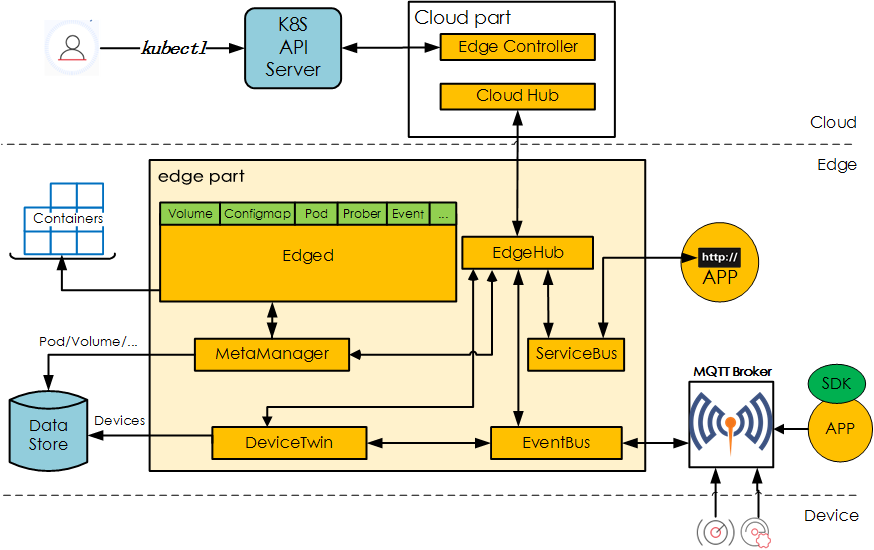
\includegraphics[width=(\textwidth+4cm)/2]{figures/kubeedge_arch.png}
    \caption{The Kubeedge system design.}
    \label{fig:kubeedgeStruct}
\end{figure}
The cloud part is built upon Kubernetes and provides support for application deployment, metadata synchronization and networking all through the Kubernetes API Server. The cloud and edge part communicate via web sockets. This means by design a good connection to the server is expected and the intend of the authors is to enable Fog computing. It is built upon Kubernetes and provides core infrastructure support for networking, application deployment and metadata synchronization between cloud and edge.\\
The edge part is not based on Kubernetes but uses similar concepts: Pods, volumes, events and more. It provides a life cycle management for containers and supports MQTT for communication for additional components. It also stores and synchronizes the device status to the cloud and has a query interface for local applications.

\subsubsection{Conclusion}
Only recently have industry behemoths like, Docker, Huawei, Bosch, Siemens, Red Hat, VMware and more\cite{K8sattheEdgeContectOnWorkingGroup:online} started to develop and, more importantly, concentrate their efforts on integrated IoT Gateway solutions. This lack of standardization is also acknowledged by the developers themselves ``While the problems at the IoT edge — connectivity, manageability, scalability, reliability, security — are being solved as point solutions by enterprises and ecosystem players, there is a need for a foundational industry-wide standard for managing distributed IoT workloads.''\cite{ioFogK8sBlog:online}\\
\Cref{tab:shortSotaSoftware} shows how the different solutions analyzed in this section compare to each other in key aspects.
% \footnote{An extended version can be found in the appendix.}
\begin{table}[h!]
% \hspace*{-2cm}
    \begin{center}
        
    \noindent\makebox[\textwidth]{
\resizebox{\columnwidth}{!}{%
\begin{tabular}{l|lll p{2.5cm} lllll}
                  & \begin{tabular}[c]{@{}l@{}}Open\\Source\end{tabular} & \begin{tabular}[c]{@{}l@{}}Centralized \\ control plane\end{tabular} & SW   &  Protocols  & \begin{tabular}[c]{@{}l@{}}System Req\\ control plane\end{tabular} & \begin{tabular}[c]{@{}l@{}}System Req\\ worker node\end{tabular} & \begin{tabular}[c]{@{}l@{}}Container\\based\end{tabular} & \begin{tabular}[c]{@{}l@{}}Kubernetes\\ in cloud\end{tabular} & \begin{tabular}[c]{@{}l@{}}Kubernetes\\ on edge\end{tabular} \\ \cline{1-10} 
Bosch IoT         & No                                                                                                                             & Yes (cloud)                                                                                                                                  & Java & ZigBee, Z-Wave, BLE and more        & Server grade                                                                                                                               & Edge grade                                                                                                                               & No                                                                                                                                & Some                                                                                                                                  & No                                                                                                                                   \\
ioFog             & Yes                                                                                                                            & Yes (cloud)                                                                                                                                  & Java & ZigBee, Z-Wave, BLE and more        & Server grade                                                                                                                               & Edge grade                                                                                                                               & Yes                                                                                                                               & Some                                                                                                                                  & No                                                                                                                                   \\
Docker\\Enterprise & No                                                                                                                             & Yes (cloud)                                                                                                                                  & Go   & ZigBee, Z-Wave, BLE and more        & Server grade                                                                                                                               & Edge grade                                                                                                                               & Yes                                                                                                                               & No                                                                                                                                    & No                                                                                                                                   \\
K3s               & Yes                                                                                                                            & Yes (both)                                                                                                                                   & Go   & Only IP based protocols             & Edge grade                                                                                                                                 & Edge grade                                                                                                                               & Yes                                                                                                                               & Yes                                                                                                                                   & Yes                                                                                                                                  \\
Kubeedge          & Yes                                                                                                                            & Yes (cloud)                                                                                                                                  & Go   & MQTT and IP. More planned & Server grade                                                                                                                               & Edge grade                                                                                                                               & Yes                                                                                                                               & Yes                                                                                                                                   & No                                                                                                                         
\end{tabular}}}
    \caption{Summary of the analyzed software.}
    \label{tab:shortSotaSoftware}
    \end{center}
\end{table}
It is important to bear in mind, that the Bosch IoT solution as well as ioFog are significantly older than the other projects. Boschs IoT solution is based on the OSGi framework. It provides isolation evolving around the JVM. This enables it to be platform independent, that is as long as the OS provides a JVM. ioFog which is almost three years old as of time of writing (June 2019) and already relays on containers, specifically a Docker runtime, for its deployment.\\
As the second last column shows all solutions, except for Docker Edge, use Kubernetes as their orchestration platform and control plane of choice. ioFog and Bosch IoT Edge are currently updating their solution while Kubeedge and K3s where designed from the ground up with Kubernetes in mind. However, only K3s tries to bring Kubernetes to the edge as well. This also means, that all solutions require different hardware requirements for the control plane, usually server grade hardware running containers, and more resource efficient solutions for the edge. \\
It is also important to note that all newer solutions, Docker Edge Solution\footnote{As the source code is not publicly available, this is speculative based on the fact that the main programming language for Docker is Go.} K3s and Kubeedge are developed in the Go programming language. Older systems are mainly based on Java as it enables code to run on every JVM supported platform. It is also important to note, that containers give developers freedom of programming language. The Bosch IoT Edge Solution and its use of the OSGi framework force developers into using a JVM compatible programming language. Docker points out that its solution runs on MacOS and Windows, however, both rely on Linux system calls.\footnote{Docker on Windows uses the WSL 2.0 in the future which translates Linux system calls to Windows system calls and increases performance a lot compared to emulated solutions as done on MacOS.}.\\
Another important aspect is protocol support. Here, the OSGi framework is clearly ahead as it has complete access to the system hardware, due to the JVM and also 



% From a design perspective, this is very similar to containers, where isolation is provided by Cspaces and Namespaces instead of process ID. Containers need access to communication 

% Giving access to devices like  Blt sigbee is a security issue.
